\documentclass[12pt, preprint]{aastex}

% words
\newcommand{\project}[1]{\textsl{#1}}
\newcommand{\thecannon}{\project{The~Cannon}} 
\newcommand{\tc}{\project{The~Cannon}} 
\newcommand{\apogee}{\project{APOGEE}}
\newcommand{\apokasc}{\project{APOKASC}}
\newcommand{\aspcap}{\project{ASPCAP}}
\newcommand{\corot}{\project{Corot}}
\newcommand{\kepler}{\project{Kepler}}
\newcommand{\gaia}{\project{Gaia}}
\newcommand{\gaiaeso}{\project{Gaia--ESO}}
\newcommand{\galah}{\project{GALAH}}
\newcommand{\most}{\project{MOST}}
\newcommand{\documentname}{\textsl{Article}}

\newcommand{\teff}{\mbox{$\rm T_{eff}$}}
\newcommand{\kms}{\mbox{$\rm kms^{-1}$}}
\newcommand{\feh}{\mbox{$\rm [Fe/H]$}}
\newcommand{\xfe}{\mbox{$\rm [X/Fe]$}}
\newcommand{\alphafe}{\mbox{$\rm [\alpha/Fe]$}}
\newcommand{\mh}{\mbox{$\rm [M/H]$}}
\newcommand{\logg}{\mbox{$\rm \log g$}}
\newcommand{\noise}{\sigma_{n\lambda}}
\newcommand{\scatter}{s_{\lambda}}
\newcommand{\pix}{\mathrm{pix}}
\newcommand{\rfn}{\mathrm{ref}}
\newcommand{\rgc}{\mbox{$\rm R_{GC}$}}
\newcommand{\vgal}{\mbox{$\rm V_{GAL}$}}

% math
\newcommand{\numax}{$\nu_{\max}$}
\newcommand{\deltanu}{$\Delta\nu$}

\begin{document}

\title{Measuring red-giant masses and ages with stellar spectra}
\author{M.~Ness\altaffilmark{1},
David~W.~Hogg\altaffilmark{1,2,3},
H.-W.~Rix\altaffilmark{1},
\textbf{others}}
\altaffiltext{1}{Max-Planck-Institut f\"ur Astronomie, K\"onigstuhl 17, D-69117 Heidelberg, Germany}
\altaffiltext{2}{Center for Cosmology and Particle Physics, Department of Phyics,
             New York University, 4 Washington Pl., room 424, New York, NY, 10003, USA}
\altaffiltext{3}{Center for Data Science, New York University, 726 Broadway, 7th Floor, New York, NY 10003, USA}
% \altaffiltext{4}{NSF Astronomy and Astrophysics Postdoctoral Fellow}
% \altaffiltext{5}{Department of Physics \& Astronomy, Johns Hopkins University, Baltimore, MD, 21218, USA}
\email{ness@mpia.de}

\begin{abstract}%
% Context
With \thecannon, we have demonstrated that it is possible to use a
small training set of stars with noisy spectral data and known
stellar-parameter labels to build a data-driven probabilistic model of
stellar spectra that can be used to infer stellar-parameter labels for
other stars (with differently noisy spectral data).
% Aims
% Method
Here we train this system using stars with known stellar mass labels
obtained from a training set of stars with both
\kepler\ asteroseismological observations (hence the known masses) and
\apogee\ infrared spectral data.
We find that (after training) \thecannon\ can infer stellar
masses---and therefore also stellar ages---for red-giant stars using
infrared spectral data alone.
% Results
We demonstrate the validity of the stellar masses and ages by three
methods:
First, we use cross-validation to demonstrate label accuracy on the
training set; we find mass accuracies of roughly XXXX and age accuracies
of roughly ZZZZ for typical-quality \apogee\ spectra.
Second, we look at the dependence on mass (or age) of
\thecannon\ spectral expectation, and show that it makes good physical
sense:
The age indicators in the spectral space are associated with elements
that can be ``dredged up'' or elements where chromospheric activity is
visible, or XXXX or YYYY.
Third, we use \thecannon\ to estimate age labels for the entire
\apogee\ sample, and show that the ages of stellar structures in the
Milky Way follow expectations, even conditioned on abundances.
All three of these tests show that we can obtain red-giant mass and
age information from stellar spectra; these capabilities open up new
opportunities for Milky Way and stellar astrophysics.
\end{abstract}

\keywords{%
keywords: incomplete (DWH)!
---
methods: data analysis
---
methods: statistical
---
stars: abundances
---
stars: fundamental parameters
---
surveys
---
techniques: spectroscopic
}

\section{Introduction}\label{sec:Intro}

Asteroseismology surveys, such as \most, \corot, and \kepler, have
been extremely successful and productive in bringing us information
about stellar interiors and (therefore) ages.
These missions operate by taking high-cadence, high-precision stellar
photometry, in which stellar oscillation modes are visible in the
Fourier domain.
These missions have operated by taking long stretches of
uninterrupted, uniform, dense imaging data on thousands of individual
stars.
They are expensive missions, but absolutely critical to calibrate
physical stellar interior models and set standards for stellar
parameter estimation, all of which is required for the ultimate
success of the next generation of stellar surveys, particularly
including the \gaia\ Mission.

At the same time, there are many large spectroscopic surveys, such
as \apogee, \galah, and \gaiaeso, underway to measure the properties
of stellar \emph{exteriors}.
These surveys will take high signal-to-noise, high resolution spectra
of hundreds of thousands of stars, revealing detailed surface chemical
abundances.

One question that naturally arises is:
How do we use these two pieces of information (surface spectroscopy
and interior asteroseismology) to jointly infer stellar properties?
Another is:
Is there any way we could learn about stellar interiors from surface
spectroscopy?
After all, at current prices, the marginal cost of taking a spectrum of
a new star is very low relative to the marginal cost of getting its
asteroseismology.
If we can determine the interior properties of stars from surface
spectroscopy alone, even noisily, great opportunities would arise for
studying the stellar populations of the Milky Way and their formation.

\ldots DWH: What are our hypotheses about how mass or age might appear
in a stellar spectrum?  It might appear as dredge-up of evolved
material from the core into the photosphere.  It might appear as
chromospheric emission from a time-dependent magnetic field.  It might
appear as line-shape variations as stellar rotation evolves.  It might
appear as amplitude variations in non-LTE effects as convection scales
are different for stars of different masses.

\ldots DWH: Importantly, age might only appear in the spectra as
certain combinations of surface abundances that are highly covariant
with age.  For example, older stars in the Milky Way tend to be more
alpha-enhanced.  We will consider such age indicators illegitimate;
the purpose of this project is to obtain estimates for ages and masses
\emph{that work even within narrow abundance-selected subsamples}.

\section{Method}

\ldots DWH: A reminder of what \thecannon\ is.

\ldots MKN: What is the training set?  How has it been selected and adjusted?

The training set of stars is a subset of 1500 stars from \citet{Martig2015}. These are \apokasc\ stars, with \numax\ and \deltanu\ measurements from \kepler, with corresponding spectra in the H-band across 1.5-1.7 $\micron$ at a resolution of R $\sim$ 22,500, observed as part of the \apogee\ survey. These stars have been selected with no warning or error in the \aspcap\ FLAG parameter provided by \apogee\ \citep{Ahn2014}, with no rotation flag set and with errors on the delta$\_$nu and nu$\_$max less than 5\%. These stars are a high Signal to Noise (SNR) sample, with an average SNR $\approx$ 330 $\pm$ 155. 

Five labels are used for training of \tc, the \teff, \logg, \feh, \alphafe\ and Mass. The training labels adopted were the \aspcap-corrected \citep{Meszaros2013} values for the \teff, \feh\ and \alphafe\ and the astroseismic value for \logg, as determined from the measured $\nu_{max}$ . The mass label was determined using the standard seismic scaling relation given in \ref{eqn1} \citep{SilvaAguirre2011,Chaplin2011}.

\begin{equation} \label{eq:mass}
M= \left( \frac{\nu_{\mathrm{max}}}{\nu_{\mathrm{max,\odot}}}\right)^3\  \left( \frac{\Delta \nu}{\Delta \nu_{\odot}}\right)^{-4} \ \left( \frac{T_{\mathrm{eff}}}{T_{\mathrm{eff,\odot}}}\right)^{1.5} \ .
\label{eq1}
\end{equation}
We adopt  $T_{\mathrm{eff,\odot}}=5777$ K, $\nu_{\mathrm{max,\odot}}=3140\ \mu$Hz, $\Delta \nu_{\odot}=135.03\ \mu$Hz. The solar values  $\Delta \nu_{\odot}$ and $\nu_{\mathrm{max,\odot}}$ are the ones used to build the APOKASC catalogue and were obtained by \cite{Hekker2013} with the OCT method. 

\section{Validation of Model}

For cross validation, we took the 


%(note this improves by 10\% from 0.27 to 0.24 if take errors on nu max and delta nu to less than 5 percent. )

%from MM:\\ 
%- error on delta$\_$nu and nu$\_$max lower than 5\% (the cut was at 10% before)\\
%- no star in the list of fast rotating stars from Jamie Tayar\\
%- no warning or error in ASPCAPFLAG\\
%- Carbon and Nitrogen abundances $>$-9999\\

\ldots MKN: Some visualization of the trained model and teasers.

\section{Experiments and Results}

\ldots MKN: What is the cross-validation and what are the results?
%plotdiff_5labels_10percent_linear_orig.py trained on 1639 stars if
%run -i plotdiff_5labels_10percent_linear trained on 1500 stars
\begin{figure}[h!]
\centering
 % \includegraphics[scale=0.31]{./plots/validation.png}
    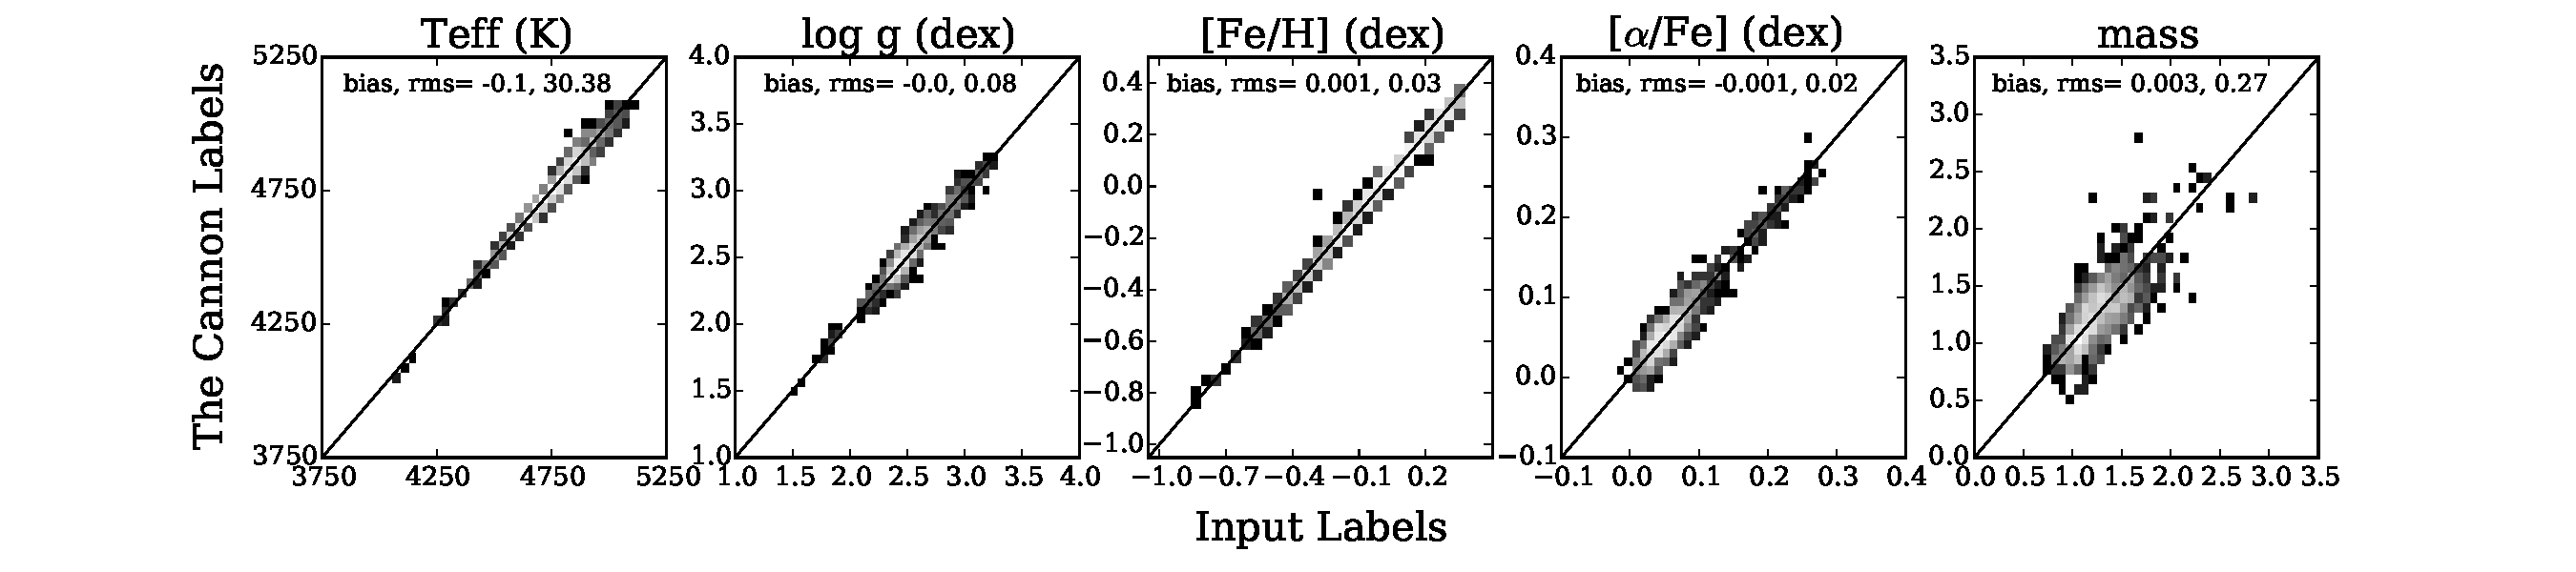
\includegraphics[scale=0.31]{./plots/validation_1500.pdf}
  \caption{Trained on 90\% of the 1639 APOKASC sample and test step on remaining 10\%, run through 10 times.}
\label{fig:validation}
\end{figure}

\ldots MKN: What are the spectral signatures of mass and how do they
map on to our hypothesized mass and age indicators?

%makeelements2.py
\begin{figure}[h!]
\centering
  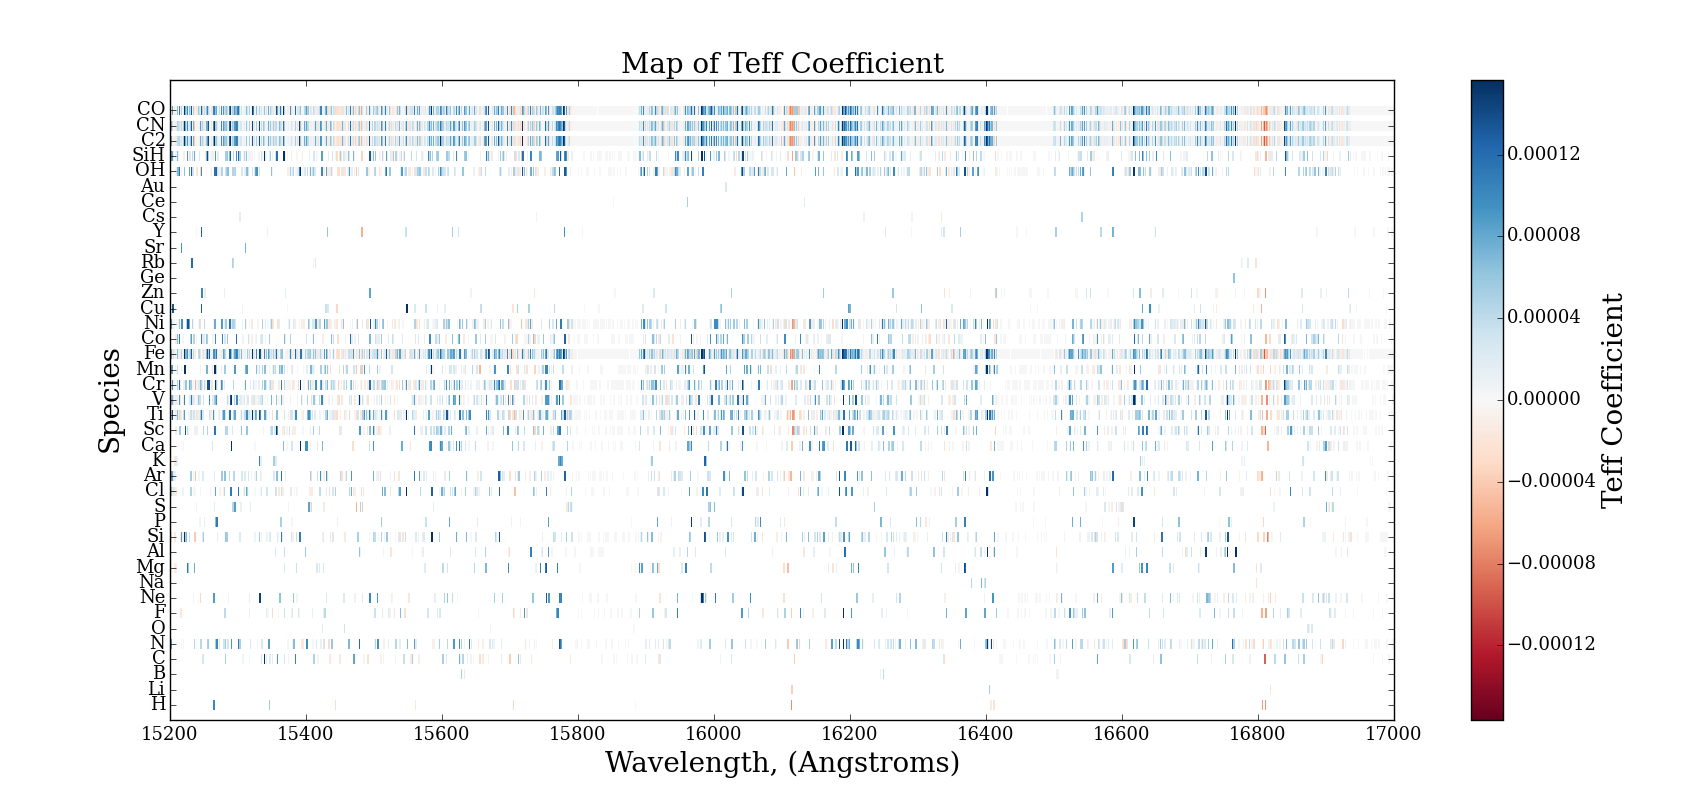
\includegraphics[scale=0.21]{./plots/teff_coefficient.png}
  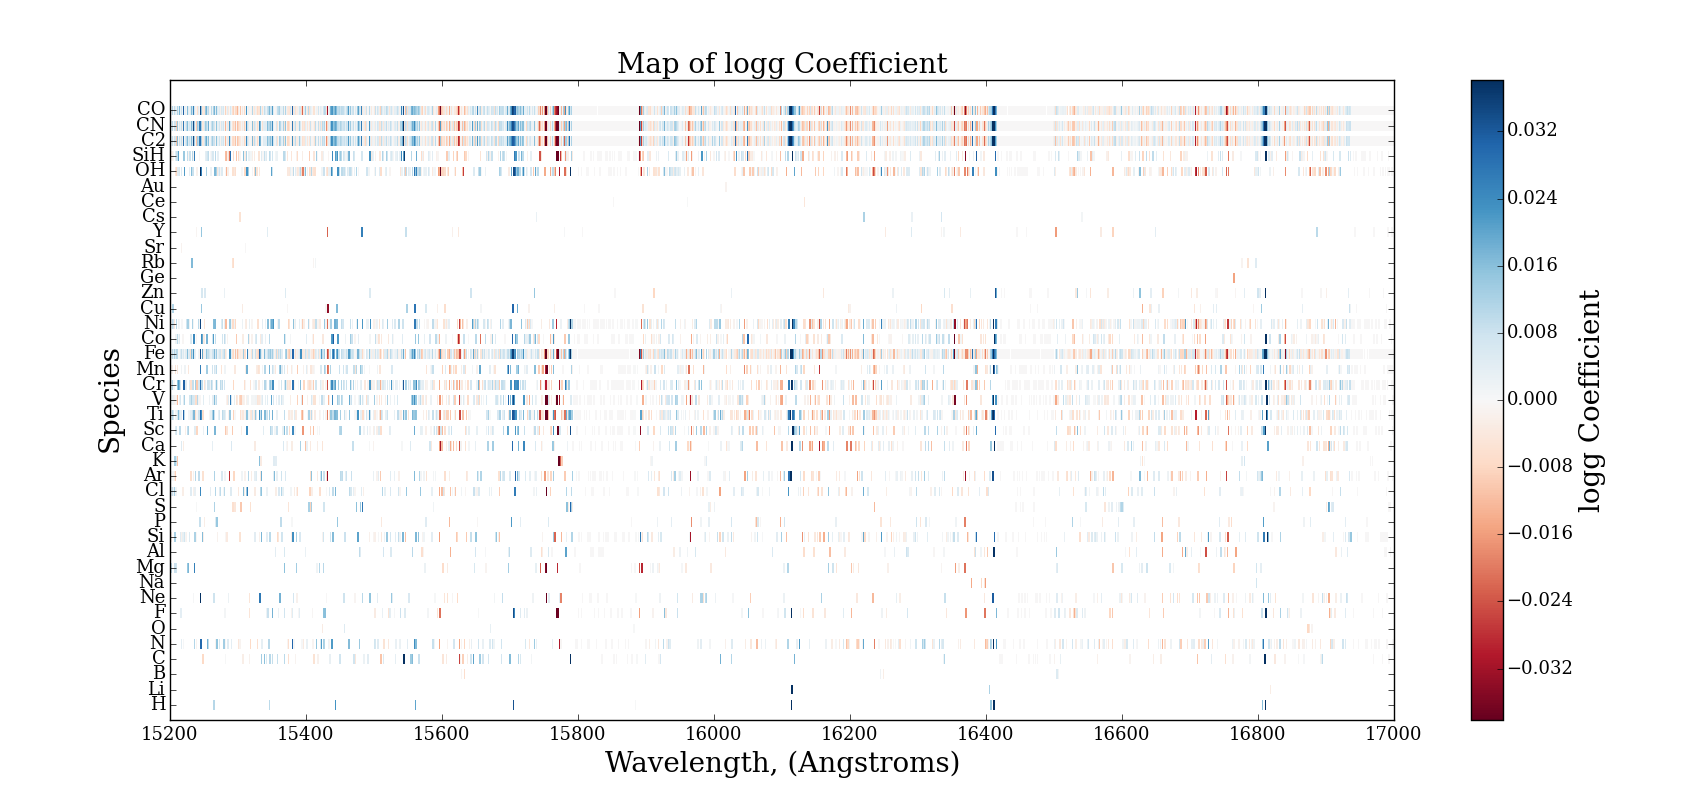
\includegraphics[scale=0.21]{./plots/logg_coefficient.png}
  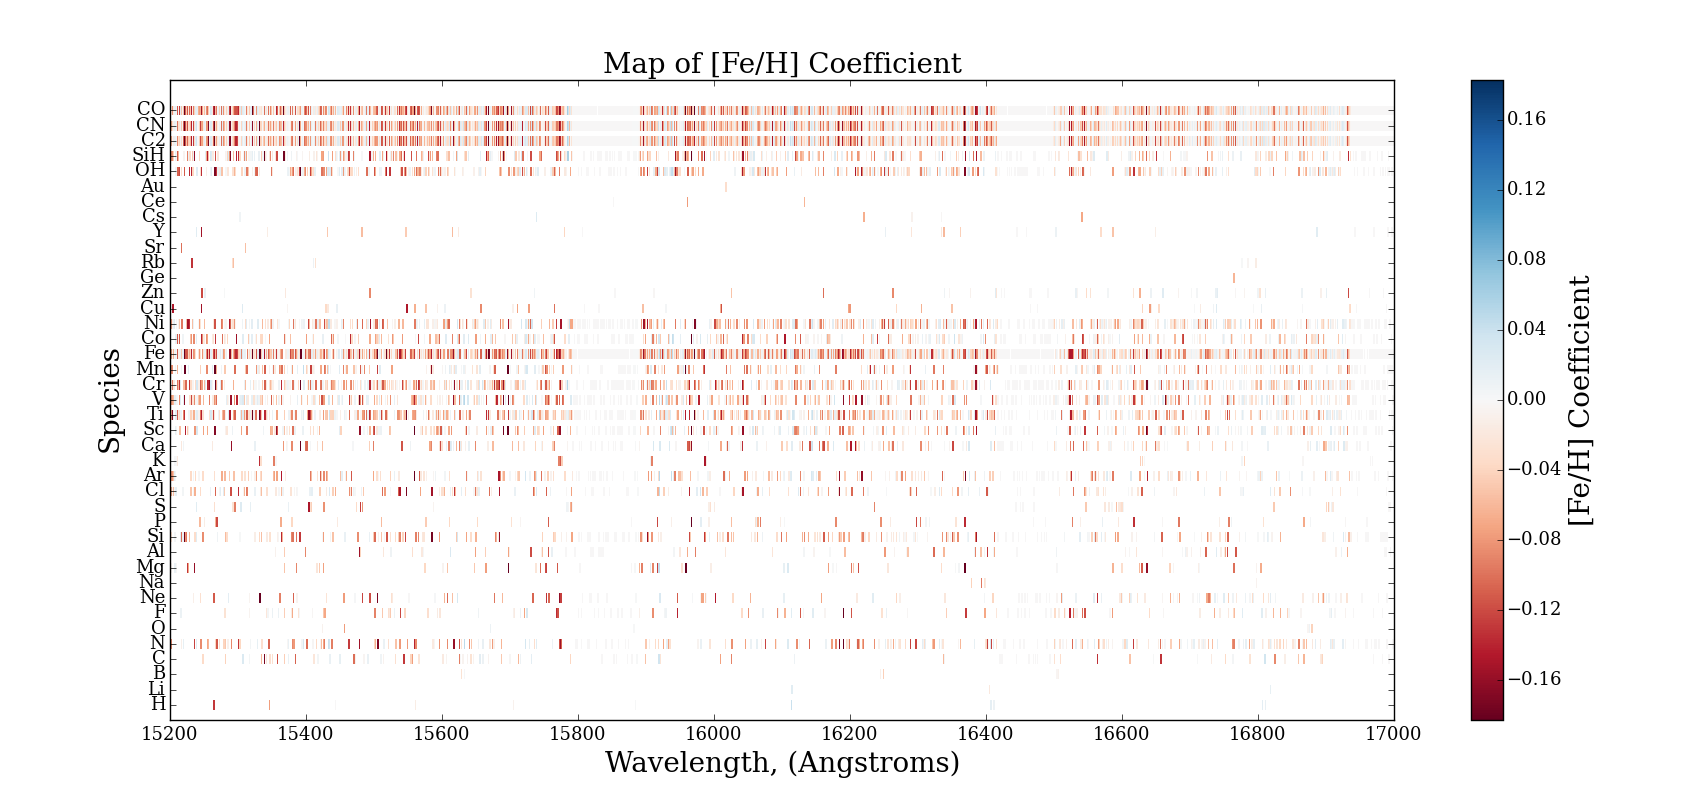
\includegraphics[scale=0.21]{./plots/feh_coefficient.png}
  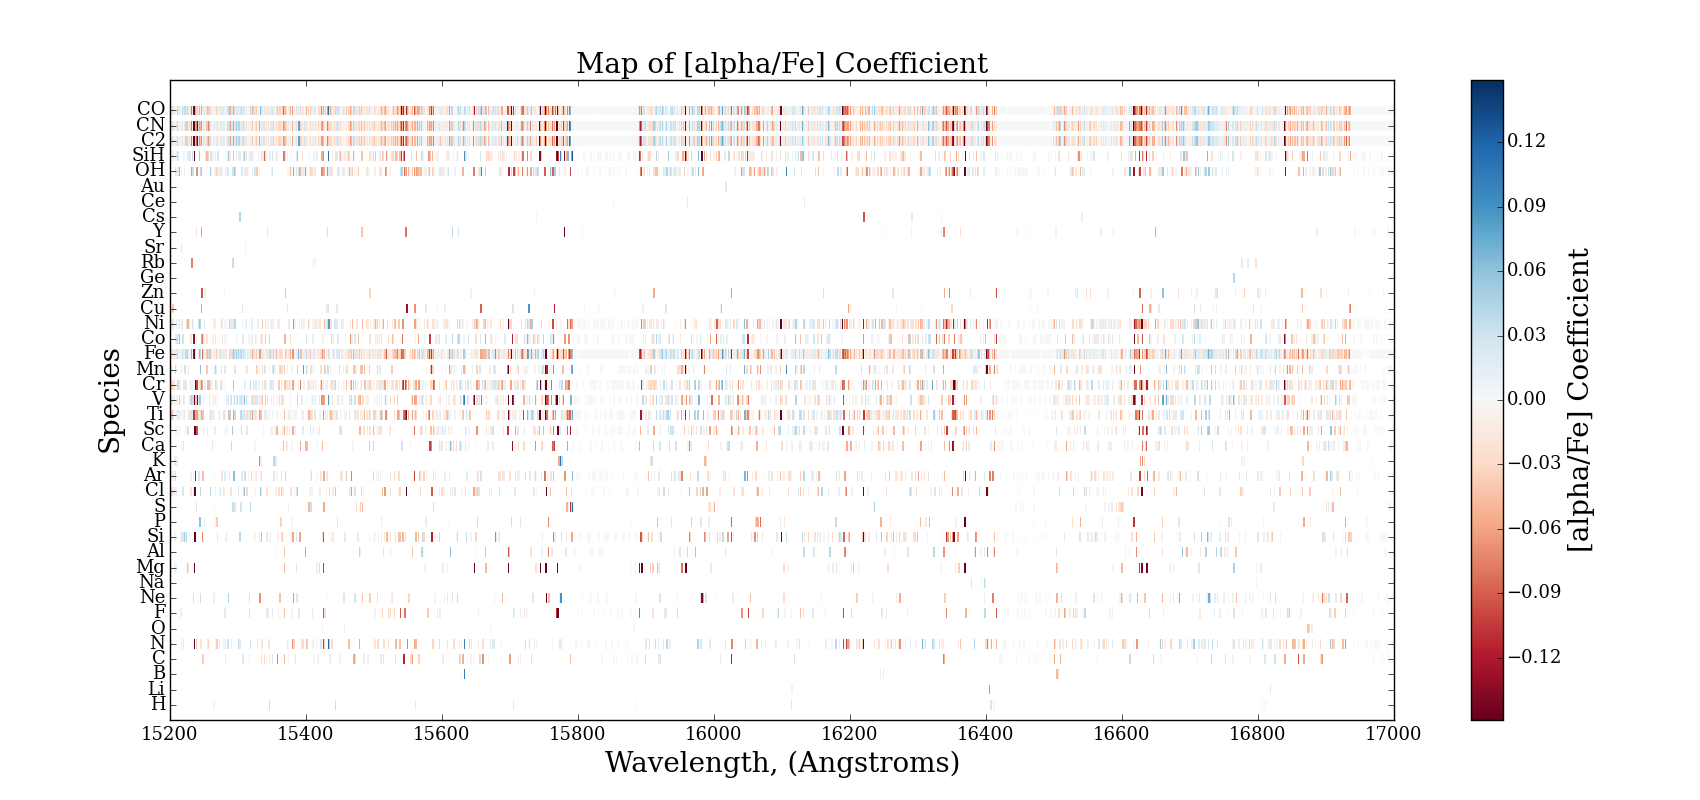
\includegraphics[scale=0.21]{./plots/alphafeh_coefficient.png}
  \includegraphics[scale=0.21]{./plots/mass_coefficient.png}
  \caption{maps} 
\label{fig:maps}
\end{figure}

\ldots MKN: What does the Galaxy look like in terms of age gradients,
in subsamples chosen for chemical homogeneity?

\section{Discussion}

\ldots DWH: Re-cap of what we have achieved and how we know we have
succeeded.

\ldots DWH: Emphasis on the reason that the science result is so
convincing that we really have an age indicator here.

\ldots MKN: What of the hypothesized age indicators are in fact
dominant?

\ldots MKN: How do you obtain our code, data, and results?

\acknowledgments
It is a pleasure to thank
  Foo,
  John Bochanski (Rider),
  Dan Foreman-Mackey (UW), and
  Bar,
for valuable discussions and contributions.
This project made use of
  The NASA Astrophysics Data System,
  and open-source code in the \project{numpy} and \project{scipy} packages.

[Insert SDSS boilerplate here.]

All code and data produced in this project is available HERE and THERE.

\end{document}
